\documentclass[11pt,a4paper]{article}

\usepackage[utf8]{inputenc}
\usepackage[T1]{fontenc}
\usepackage{geometry}
\usepackage{titlesec}
\usepackage{graphicx}
\usepackage{float}
\usepackage{xcolor}
\usepackage{listings}
\usepackage{hyperref}
\usepackage{enumitem}

\geometry{margin=2.5cm}

\hypersetup{
    colorlinks=true,
    linkcolor=blue,
    urlcolor=blue
}

\titleformat{\section}
{\large\bfseries}
{\thesection.}{0.5em}{}

\titleformat{\subsection}
{\normalsize\bfseries}
{\thesubsection.}{0.5em}{}

\definecolor{codebg}{rgb}{0.95,0.95,0.95}

\lstset{
    backgroundcolor=\color{codebg},
    basicstyle=\ttfamily\small,
    frame=single,
    breaklines=true,
    columns=fullflexible
}

\begin{document}

\begin{titlepage}
    \centering

    \vspace*{3cm}

    {\Huge \textbf{Linux Storage Management and LVM}}\\[1cm]

    {\Large Server Engineering Labs}\\[2cm]

    \textbf{Author:}\\
    Laura Ortiz Moreno\\[1cm]

    \textbf{Topics Covered:}
    \begin{itemize}[leftmargin=4cm]
        \item Linux storage administration
        \item Partition management
        \item Logical Volume Management (LVM)
        \item Filesystem migration
        \item Persistent mounts with \texttt{fstab}
    \end{itemize}

    \vfill

    \textbf{Environment:}\\
    Debian Linux Virtual Machine\\
    Virtualized lab environment

    \vspace{1cm}

\end{titlepage}

\tableofcontents
\newpage

\section{Introduction}

This report documents several Linux storage administration tasks performed in a virtualized Debian environment. The main objective was to understand how Linux handles disks, partitions, mount points, and Logical Volume Management (LVM).

The exercises focused on:
\begin{itemize}
    \item Detecting and managing storage devices
    \item Creating and mounting partitions
    \item Configuring LVM structures
    \item Migrating directories such as \texttt{/var}
    \item Making mounts persistent through \texttt{/etc/fstab}
\end{itemize}

The work was carried out in a controlled laboratory environment using virtual machines.

\section{Disk Detection and Initial Inspection}

The first step consisted of inspecting the disks detected by the operating system.

Useful commands included:

\begin{lstlisting}[language=bash]
lsblk
fdisk -l
df -h
\end{lstlisting}

These commands allow the administrator to:
\begin{itemize}
    \item Identify physical disks
    \item Check existing partitions
    \item Verify mounted filesystems
    \item Inspect storage usage
\end{itemize}

\begin{figure}[H]
    \centering
    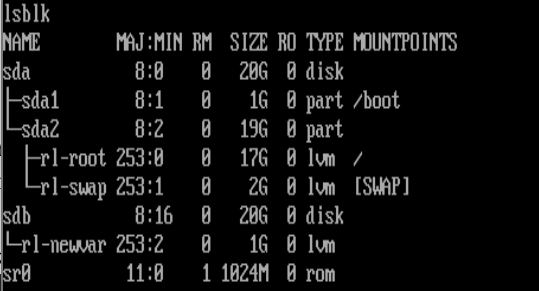
\includegraphics[width=0.78\textwidth]{images/lvm/lsblk-initial-lvm.png}
    \caption{Initial disk layout and LVM structure shown using \texttt{lsblk}.}
\end{figure}

\section{Creating and Managing Partitions}

A new partition was created in order to prepare additional storage for LVM.

Typical workflow:

\begin{lstlisting}[language=bash]
sudo fdisk /dev/sdb
\end{lstlisting}

Inside \texttt{fdisk}, the partition table was modified and a new Linux partition was created.

After saving the changes, the partition table was reloaded:

\begin{lstlisting}[language=bash]
sudo partprobe
\end{lstlisting}

The partition was then formatted:

\begin{lstlisting}[language=bash]
sudo mkfs.ext4 /dev/sdb1
\end{lstlisting}

\section{Logical Volume Management (LVM)}

The laboratory also introduced the use of LVM for flexible storage administration.

The process included:
\begin{enumerate}
    \item Creating a Physical Volume (PV)
    \item Creating a Volume Group (VG)
    \item Creating a Logical Volume (LV)
    \item Formatting and mounting the LV
\end{enumerate}

\subsection{Creating the Physical Volume}

\begin{lstlisting}[language=bash]
sudo pvcreate /dev/sdb1
\end{lstlisting}

\subsection{Creating the Volume Group}

\begin{lstlisting}[language=bash]
sudo vgcreate vg_data /dev/sdb1
\end{lstlisting}

\subsection{Creating the Logical Volume}

\begin{lstlisting}[language=bash]
sudo lvcreate -L 5G -n lv_var vg_data
\end{lstlisting}

\subsection{Formatting the Logical Volume}

\begin{lstlisting}[language=bash]
sudo mkfs.ext4 /dev/vg_data/lv_var
\end{lstlisting}

\section{Migrating the \texttt{/var} Directory}

One of the most important tasks was migrating the \texttt{/var} directory into the new logical volume.

The migration process required:
\begin{itemize}
    \item Creating a temporary mount point
    \item Copying all files while preserving permissions
    \item Updating \texttt{/etc/fstab}
    \item Rebooting and validating the configuration
\end{itemize}

\subsection{Temporary Mount}

\begin{lstlisting}[language=bash]
sudo mkdir /mnt/var_temp
sudo mount /dev/vg_data/lv_var /mnt/var_temp
\end{lstlisting}

\subsection{Copying Files}

\begin{lstlisting}[language=bash]
sudo rsync -av /var/ /mnt/var_temp/
\end{lstlisting}

\begin{figure}[H]
    \centering
    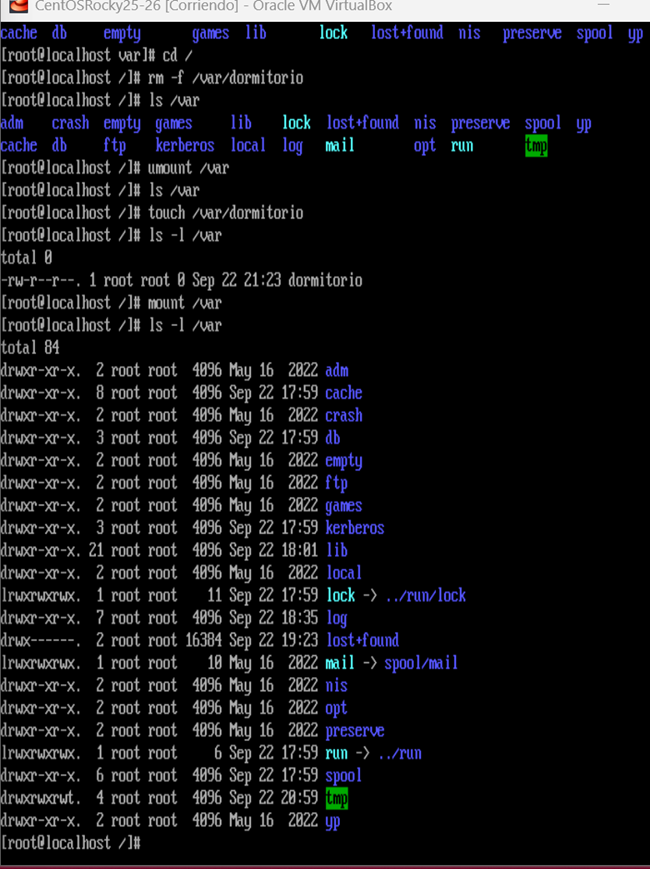
\includegraphics[width=0.92\textwidth]{images/lvm/mount-validation.png}
    \caption{Validation of the temporary \texttt{/var} mount and filesystem behavior after unmounting and remounting operations.}
\end{figure}

\subsection{Persistent Mount Configuration}

The filesystem was added to \texttt{/etc/fstab}:

\begin{lstlisting}
UUID=<uuid> /var ext4 defaults 0 2
\end{lstlisting}

\section{Verification and Validation}

After rebooting the system, the configuration was verified using:

\begin{lstlisting}[language=bash]
mount | grep var
df -h
lsblk
\end{lstlisting}

\begin{figure}[H]
    \centering
    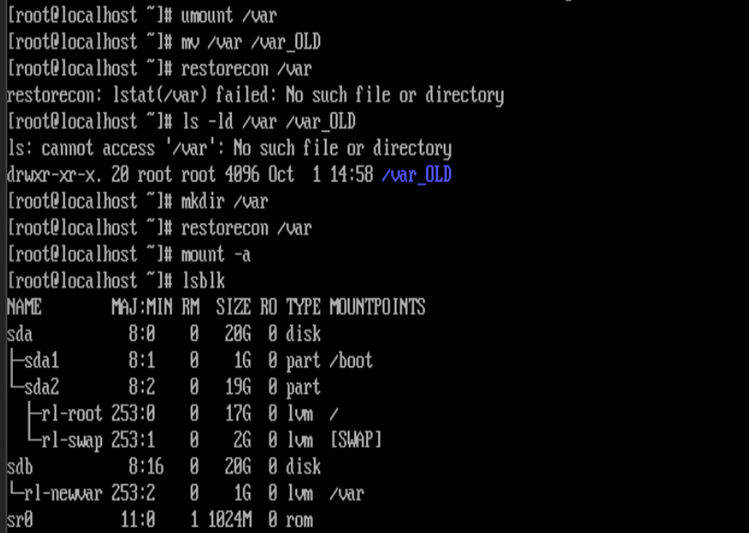
\includegraphics[width=0.82\textwidth]{images/lvm/final-var-mount.png}
    \caption{Final LVM configuration after mounting the logical volume on \texttt{/var}.}
\end{figure}

The logical volume was successfully mounted and persisted correctly after reboot.

\section{Challenges Encountered}

Several issues appeared during the lab:
\begin{itemize}
    \item Incorrect mount configurations
    \item Filesystem permission inconsistencies
    \item Risks when modifying \texttt{/etc/fstab}
\end{itemize}

Particular care had to be taken because incorrect \texttt{fstab} entries can prevent Linux from booting correctly.

\section{Conclusion}

This laboratory provided practical experience with Linux storage administration and LVM management.

The exercises demonstrated:
\begin{itemize}
    \item How Linux organizes storage devices
    \item How logical volumes improve flexibility
    \item How to safely migrate important directories
    \item The importance of persistent filesystem configuration
\end{itemize}

These concepts are essential for Linux system administration, server deployment, and infrastructure management.

\end{document}